
% !TEX encoding = UTF-8 Unicode 
% !TEX root = FieldGuide.tex

\Sec{Beta Prime Distribution}
\label{sec:BetaPrime}



\dist{Beta prime} (beta type II, Pearson type VI, inverse beta, variance ratio, gamma ratio, compound gamma, $\beta'$) distribution~\cite{Pearson1901,Johnson1995}:
\begin{align}
\label{BetaPrime}
\opr{BetaPrime}&(x\given  a, s,\alpha, \gamma) \\ \notag&= \frac{1}{B(\alpha,\gamma)}\frac{1}{|s|} \Left(\frac{x-a}{s}\Right)^{\alpha -1} \Left(1+\frac{x-a}{s}\Right)^{-\alpha-\gamma }  \checked
\\
&= \opr{GenBetaPrime}(x\given a,s, \alpha,\gamma,1) \notag \checked
\\
& \text{for }  a,\ s,\ \alpha,\ \gamma \text{ in } \Real, \  \alpha>0, \gamma>0  \checked
\notag \\ 
& \text{support } x \geq a \ \text{if}\ s > 0,  \ x\leq a  \ \text{if}\  s < 0 
\notag
\end{align}
A Pearson distribution~\secref{sec:Pearson} with semi-infinite support, and both roots on the real line. Arises notable as the ratio of gamma distributions, and as the order statistics of the uniform-prime distribution~\eqref{UniPrime}.



\SSec{Special cases}
Special cases of the beta prime distribution are listed in table~\ref{GenBetaPrimeTable}, under $\beta=1$.


\dist{Standard beta prime} (beta prime) distribution~\cite{Pearson1901}:
\begin{align}
\label{StdBetaPrime}
\opr{StdBetaPrime}(x\given \alpha, \gamma) &= \frac{1}{B(\alpha,\gamma)} x^{\alpha -1} (1+x )^{-\alpha-\gamma } \checked
\\&= \opr{BetaPrime}(x\given  0,1, \alpha,\gamma) \notag	\checked
\\&= \opr{GenBetaPrime}(x\given  0,1, \alpha,\gamma,1) \notag \checked
\end{align}


\begin{figure}[tp!]
\begin{center}
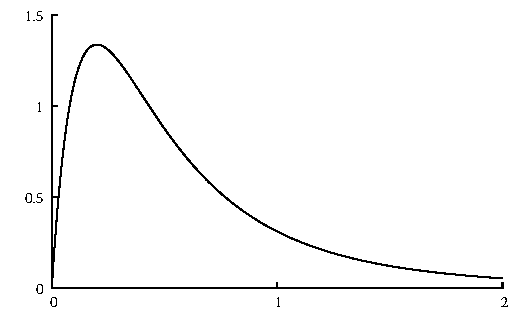
\includegraphics[width=\textwidth]{pdfBetaPrime}
\end{center}
\caption[Beta prime distribution]{A beta prime distribution, $\opr{BetaPrime}(0, 1, 2, 4)$}
\end{figure}


\dist{F} (Snedecor's F, Fisher-Snedecor, Fisher, Fisher-F, variance-ratio, F-ratio) distribution~\cite{Snedecor1934, Aroian1941, Johnson1995}:
\begin{align}
\label{F}
\opr{F}(x\given k_1,k_2) &= \frac{k_1^{\tfrac{k_1}{2} }   k_2^{\tfrac{k_2}{2}}}{ B(\tfrac{k_1}{2}, \tfrac{k_2}{2})    }
 \frac{x^{\tfrac{k_1}{2} -1}}{(k_2 + k_1 x)^{\tfrac{1}{2}(k_1+k_2)}} \checked
 \\ & =  \opr{BetaPrime}(x\given  0,\tfrac{k_2}{k_1}, \tfrac{k_1}{2},\tfrac{k_2}{2}) \notag \checked
 \\ & =  \opr{GenBetaPrime}(x\given  0,\tfrac{k_2}{k_1}, \tfrac{k_1}{2},\tfrac{k_2}{2},1) \checked
 \notag
\\ & \text{for positive integers } k_1,\ k_2 \notag \checked
\end{align}
An alternative parameterization of the beta prime distribution that derives from the ratio of two chi-squared distributions \eqref{ChiSqr} with $k_1$ and $k_2$ degrees of freedom.
\[
\opr{F}(k_1,k_2) \sim \frac{\opr{ChiSqr}(k_1) / k_1 }{\opr{ChiSqr}(k_2) / k_2} \checked
\notag
\]



\dist{Inverse Lomax} (inverse Pareto) distribution~\cite{Kleiber2003}: 
\begin{align}
\label{InvLomax}
\opr{InvLomax}(x\given a, s,\alpha) &= \frac{\alpha}{|s|} \Left(\frac{x-a}{s}\Right)^{\alpha -1} \Left(1+\frac{x-a}{s}\Right)^{-\alpha-1} \checked
\\ \notag &= \opr{BetaPrime}(x\given a, s, \alpha,1) \checked
\\ \notag &= \opr{GenBetaPrime}(x\given a, s, \alpha,1,1) \checked
\end{align}


\begin{figure}[tp!]
\begin{center}
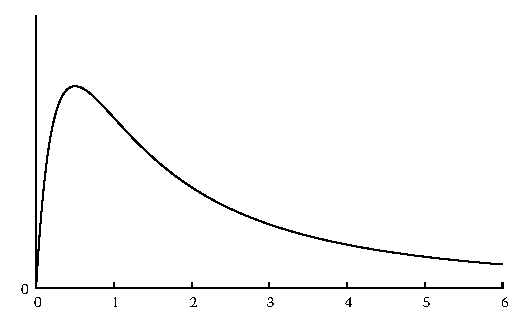
\includegraphics[width=\textwidth]{pdfInverseLomax}
\end{center}
\caption[Inverse Lomax distribution]{An inverse lomax distribution, $\opr{InvLomax}(0, 1, 2)$}
\end{figure}



% !TEX encoding = UTF-8 Unicode 
% !TEX root = FieldGuide.tex

\begin{table*}[tp]
\caption[Beta prime distribution -- Properties] {Properties of the beta prime distribution}
\begin{align*}
 \text{\hyperref[PropertiesSec]{Properties}}  \quad& \\
\text{notation} \quad & \op{BetaPrime}(x\given a, s, \alpha,\gamma)  	\checked
\\
\text{PDF}\quad &    \frac{1}{B(\alpha, \gamma)} \frac{1}{|s|}
\Left(\frac{x-a}{s}\Right)^{\alpha -1} \Left(1+ \frac{x-a}{s} \Right)^{-\alpha-\gamma } \checked
\hspace{-2em}
\\
\text{CDF / CCDF} \quad  &  
\frac{B\big(\alpha, \gamma; (1+(\tfrac{x-a}{s})^{-1})^{-1} \big) }{B(\alpha,\gamma)} \checked
\hspace{-8em}
& s >0 \,\big/ \, s<0
\\ 
& \quad = I\Left(  \alpha,\gamma; (1+(\tfrac{x-a}{s})^{-1})^{-1} \Right) 			\checked
\\
\text{parameters}\quad &   a,\ s,\ \alpha,\ \gamma, \text{ in } \Real \checked 
\\ & \alpha>0, \gamma>0 \checked
\\
\text{support} \quad &    x \geq a &  s > 0 			\checked
\\
&  x\leq a  &  s < 0 							\checked
\\
%\text{median} \quad  &  \cdots
%\\
\text{mode} \quad  & a + s \frac{\alpha-1}{\gamma+1} & \alpha\geq 1 \checked \\
& a &\alpha<1 \checked
\\
\text{mean} \quad  &   a+s \frac{ \alpha}{\gamma-1} \checked
& \gamma >1
\\
\text{variance} \quad  &s^2
\frac{\alpha(\alpha+\gamma-1)}{(\gamma-2)(\gamma-1)^2} \checked
  \hspace{-8em}
&   \gamma>2
\\
\text{skew} \quad  &  \text{not simple}
\\
\text{kurtosis} \quad  &  \text{not simple}
\\
\text{entropy} \quad  &   \ln \frac{1}{B(\alpha, \gamma)} \Left|\frac{1}{s}\Right|
  +(1-\alpha) \big[ \psi(\alpha) - \psi(\gamma)\big]
  \hspace{-8em}
\\
& \quad +(\alpha+\gamma) \big[ \psi(\alpha+\gamma) - \psi(\gamma)\big] \checked &  \text{\cite[Eq.~(15)]{Tahmasebi2010}}
\\
\text{MGF} \quad  &  \text{none}
%\\
%\text{CF} \quad  &  \cdots 
% Possible expression in terms of second confluence hypergeometric function?
% See wikipedia under F distribution
%\\
%\text{moments} \quad & \frac{B(\alpha+k,\gamma-k)}B(\alpha,\gamma)}
% Only if a =0, s=1. How do moments scale with scale?
\end{align*}
\end{table*}






\SSec{Interrelations}

The standard beta prime distribution is closed under inversion.
\[
\opr{StdBetaPrime}(\alpha,\gamma) \sim \frac{1}{\opr{StdBetaPrime}(\gamma,\alpha)} \checked
\notag
\]


The beta and beta prime distributions are related by the transformation~\secref{transforms}
\[
\opr{StdBetaPrime}(\alpha,\gamma) \sim \Left( \frac{1}{\opr{StdBeta}(\alpha,\gamma)}  -1 \Right)^{-1} \checked
\notag
\]
and, therefore, the generalized beta prime can be realized as a transformation of the standard beta \eqref{StdBeta} distribution.
\[
\opr{GenBetaPrime}(a,s,\alpha,\gamma,\beta) \sim a+ s\Left( \opr{StdBeta}(\alpha,\gamma)^{-1} -1\Right)^{-\sfrac{1}{\beta}}
\checked
\notag
\]


If the scale parameter of a gamma distribution \eqref{Gamma} is also gamma distributed, the resulting compound distribution is beta prime~\cite{Dubey1970}.
\[
\opr{BetaPrime}(0,s,\alpha,\gamma) \sim  \opr{Gamma}_2\bigl(0, \opr{Gamma}_1(0, s, \gamma),\alpha \bigr) \checked
\notag
\]
The name {\bf compound gamma} distribution is occasionally used for the anchored beta prime distribution (scale parameter, but no location parameter)

The beta prime distribution is a special case of both the generalized beta~\eqref{GenBeta} and generalized beta prime~\eqref{GenBetaPrime} distributions, and itself limits to the gamma~\eqref{Gamma} and inverse gamma~\eqref{InvGamma} distributions.
\[
\opr{Gamma}(x\given 0, \theta,\alpha)  
\notag
& =
\lim_{\gamma\rightarrow\infty} \opr{BetaPrime}(x\given 0, \theta \gamma ,\alpha, \gamma ) \checked
\\
\opr{InvGamma}(x\given \theta,\alpha) 
& =
\lim_{\gamma\rightarrow\infty} \opr{BetaPrime}(x\given 0, \theta/ \gamma ,\alpha, \gamma )  \checked
\notag
\]





